\documentclass[tikz]{standalone}
% ------- TikZ Preamble -------
\RequirePackage{tikz}
\usetikzlibrary{knots,hobby,calc,intersections,decorations.pathreplacing,shapes.geometric,spath3}

% ------- Shared styles (from your preamble) -------
\tikzset{
    knot diagram/every strand/.append style={ultra thick, black},
%               every path/.style={black,line width=2pt},
%               every node/.style={transform shape,knot crossing,inner sep=1.5pt},
%               every knot/.style={line cap=round,line join=round,very thick},
%               strand/.style={line cap=round,line join=round,line width=3pt,draw=black},
%               over/.style={preaction={draw=white,line width=6.5pt}},
%               sst/ring A/.style={draw=black, line width=3pt},
%               sst/ring B/.style={draw=black,  line width=3pt},
%               sst/ring C/.style={draw=black, line width=3pt},
}

% ------- Guides toggle -------
\newif\ifsstguides
\sstguidestrue

% ------- Helper: label & skeleton for points P1..Pn -------
\newcommand{\SSTGuidesPoints}[2]{% #1=basename (e.g. P), #2=last index
  \ifsstguides
    \foreach \i in {1,...,#2}{
      \fill[blue] (#1\i) circle (1.2pt);
      \node[blue,font=\scriptsize,above] at (#1\i) {\i};
    }
    \draw[gray!40, dashed]
    \foreach \i [remember=\i as \lasti (initially 1)] in {2,...,#2,1} { (#1\lasti)--(#1\i) };
  \fi
}

\usetikzlibrary{decorations.markings}
\usetikzlibrary{calc}
\usetikzlibrary{decorations.pathmorphing} % for snake/sine decoration
\usepackage{tikz}
\usepackage{tikzlings} % not required; just ensure no extras loaded
\usetikzlibrary{
    spath3,
    intersections,
    arrows,
    knots,
    calc,
    hobby,
    decorations.pathreplacing,
    shapes.geometric,
}
   % the knot package



\begin{document}
%\begin{tikzpicture}[use Hobby shortcut, line cap=round, line join=round, scale=1.0]
%
%% ====== controls ======
%\def\Amp{0.09}          % normal offset amplitude of each strand
%\def\Turns{8}           % twist periods around the full loop (visual)
%\def\Samples{200}       % total sample points (smoothness)
%\def\Wth{2.5pt}         % strand line width
%\def\OverMask{3.2pt}    % overpass mask width (should be > \Wth)
%\def\ClrA{blue!80!black}
%\def\ClrB{red!75!black}
%
%% ====== your centerline control points ======
%\coordinate (P1) at (-2.0,-2.0);  % start/close
%\coordinate (P2) at (-2.0, 2.0);
%\coordinate (P3) at ( 1.0,-0.5);
%\coordinate (P4) at (-1.0,-0.5);
%\coordinate (P5) at ( 2.0, 2.0);
%\coordinate (P6) at ( 2.0,-2.0);
%\coordinate (P7) at (-1.0, 0.5);
%\coordinate (P8) at ( 1.0, 0.5);
%\coordinate (P9) at (-2.0,-2.0);  % = P1
%
%\def\KPATH{([closed] P1)..(P2)..(P3)..(P4)..(P5)..(P6)..(P7)..(P8)..(P9)}
%
%% ====== build two offset coordinate lists A_i and B_i ======
%% local frame at position s: x=tangent, y=left-normal; place points at (0, yoffset)
%\newcommand{\MakeStrandCoords}[5]{%
%% #1 path, #2 N, #3 amplitude, #4 turns, #5 prefix (A or B)
%    \pgfmathtruncatemacro{\Ns}{#2}
%    \def\Phase{0}%
%    \ifx#5B\def\Phase{0.5}\fi % half-period shift for B
%    \foreach \i in {0,...,\Ns}{%
%        \pgfmathsetmacro{\s}{\i/\Ns}%
%        \pgfmathsetmacro{\y}{#3*sin(360*(#4*\s + \Phase))}%
%        \path[
%            postaction={
%                decorate,
%                decoration={markings, mark=at position \s with {\coordinate (#5\i) at (0,\y);}}
%            }
%        ] #1;
%    }%
%}
%\MakeStrandCoords{\KPATH}{\Samples}{\Amp}{\Turns}{A}
%\MakeStrandCoords{\KPATH}{\Samples}{\Amp}{\Turns}{B}
%
%% ====== helper to draw one cubic-arc segment between consecutive indices ======
%\newcommand{\drawSeg}[4]{% name, i, color, over(0/1)
%% #1=A/B, #2=index, #3=color, #4=over flag
%    \ifnum#4=1
%    \draw[draw=#3, line width=\Wth,
%        preaction={draw=white, line width=\OverMask}]
%    (#1#2) .. (#1\the\numexpr#2+1\relax);
%    \else
%        \draw[draw=#3, line width=\Wth]
%        (#1#2) .. (#1\the\numexpr#2+1\relax);
%    \fi
%}
%
%% ====== alternate over/under every half turn ======
%% half-turn segment length in samples:
%\pgfmathtruncatemacro{\SegN}{round(\Samples/(2*\Turns))}
%% loop over segments
%\pgfmathtruncatemacro{\Last}{\Samples-1}
%\foreach \k in {0,...,\Last}{
%    % find which half-turn segment we are in
%    \pgfmathtruncatemacro{\blk}{floor(\k/\SegN)}
%    % even blocks: A over, odd blocks: B over
%    \ifodd\blk
%    % B over, A under
%    \drawSeg{A}{\k}{\ClrA}{0}
%    \drawSeg{B}{\k}{\ClrB}{1}
%    \else
%    % A over, B under
%        \drawSeg{B}{\k}{\ClrB}{0}
%        \drawSeg{A}{\k}{\ClrA}{1}
%    \fi
%}
%
%% (Optional) faint dashed centerline:
%%\draw[gray!35, dashed, line width=0.5pt] \KPATH;
%
%\end{tikzpicture}
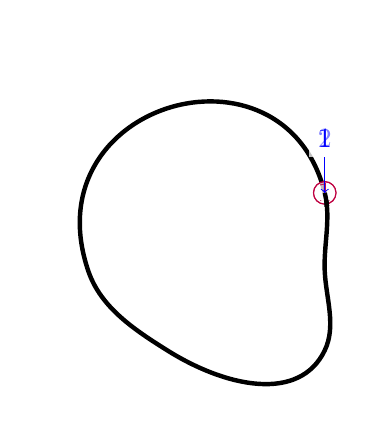
\begin{tikzpicture}[use Hobby shortcut]
    \coordinate (P1) at (1, 2);
    \coordinate (P2) at (1, 1);
    \coordinate (P3) at (1, 0);
    \coordinate (P4) at (-1, 0);
    \coordinate (P5) at (-2, 1);
    \coordinate (P6) at (1, 2); % = P1

    \begin{knot}[
        consider self intersections,
        clip width=5pt, clip radius=3pt,
        ignore endpoint intersections=false,
        draft mode=crossings % uncomment to see numbers
    ]
    \strand
    ([closed] P1)..(P2)..(P3)..(P4)..(P5)..(P6);
    \end{knot}

\end{tikzpicture}

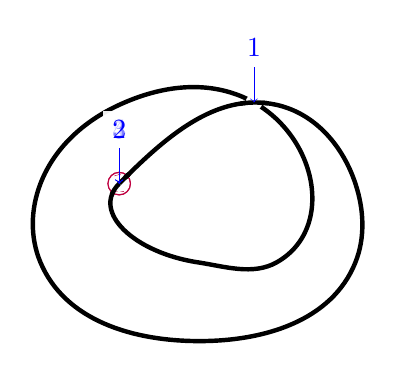
\begin{tikzpicture}[use Hobby shortcut]

    \coordinate (P1) at (-3, 1);
    \coordinate (P2) at (-1, 2);
    \coordinate (P3) at (0, 1);
    \coordinate (P4) at (0, 0);
    \coordinate (P5) at (-2, -1);
    \coordinate (P6) at (-4, 0);
    \coordinate (P7) at (-4, 1);
    \coordinate (P8) at (-3, 2);
    \coordinate (P9) at (-1, 0);
    \coordinate (P10) at (-2, 0);
    \coordinate (P11) at (-3, 1);
    \coordinate (P12) at (-3, 1); % = P1

    \begin{knot}[
        consider self intersections,
        clip width=5pt, clip radius=3pt,
        ignore endpoint intersections=false,
        draft mode=crossings % uncomment to see numbers
    ]
    \strand
    ([closed] P1)..(P2)..(P3)..(P4)..(P5)..(P6)..(P7)..(P8)..(P9)..(P10)..(P11)..(P12);
    \end{knot}

\end{tikzpicture}

\end{document}